\documentclass[conference]{IEEEtran}
\usepackage{multirow}
% \usepackage{epstopdf}
\usepackage{graphicx}
\usepackage{subfigure}
\usepackage{booktabs}
\usepackage{diagbox}
\hyphenation{Context-aware Sequential Recommendation}


\begin{document}
%
% paper title
% Titles are generally capitalized except for words such as a, an, and, as,
% at, but, by, for, in, nor, of, on, or, the, to and up, which are usually
% not capitalized unless they are the first or last word of the title.
% Linebreaks \\ can be used within to get better formatting as desired.
% Do not put math or special symbols in the title.
\title{Context-aware Sequential Recommendation}


% author names and affiliations
% use a multiple column layout for up to three different
% affiliations
\author{\IEEEauthorblockN{Michael Shell}
\IEEEauthorblockA{School of Electrical and\\Computer Engineering\\
Georgia Institute of Technology\\
Atlanta, Georgia 30332--0250\\
Email: http://www.michaelshell.org/contact.html}
\and
\IEEEauthorblockN{Homer Simpson}
\IEEEauthorblockA{Twentieth Century Fox\\
Springfield, USA\\
Email: homer@thesimpsons.com}
\and
\IEEEauthorblockN{James Kirk\\ and Montgomery Scott}
\IEEEauthorblockA{Starfleet Academy\\
San Francisco, California 96678--2391\\
Telephone: (800) 555--1212\\
Fax: (888) 555--1212}}

% conference papers do not typically use \thanks and this command
% is locked out in conference mode. If really needed, such as for
% the acknowledgment of grants, issue a \IEEEoverridecommandlockouts
% after \documentclass

% for over three affiliations, or if they all won't fit within the width
% of the page, use this alternative format:
%
%\author{\IEEEauthorblockN{Michael Shell\IEEEauthorrefmark{1},
%Homer Simpson\IEEEauthorrefmark{2},
%James Kirk\IEEEauthorrefmark{3},
%Montgomery Scott\IEEEauthorrefmark{3} and
%Eldon Tyrell\IEEEauthorrefmark{4}}
%\IEEEauthorblockA{\IEEEauthorrefmark{1}School of Electrical and Computer Engineering\\
%Georgia Institute of Technology,
%Atlanta, Georgia 30332--0250\\ Email: see http://www.michaelshell.org/contact.html}
%\IEEEauthorblockA{\IEEEauthorrefmark{2}Twentieth Century Fox, Springfield, USA\\
%Email: homer@thesimpsons.com}
%\IEEEauthorblockA{\IEEEauthorrefmark{3}Starfleet Academy, San Francisco, California 96678-2391\\
%Telephone: (800) 555--1212, Fax: (888) 555--1212}
%\IEEEauthorblockA{\IEEEauthorrefmark{4}Tyrell Inc., 123 Replicant Street, Los Angeles, California 90210--4321}}




% use for special paper notices
%\IEEEspecialpapernotice{(Invited Paper)}




% make the title area
\maketitle

% As a general rule, do not put math, special symbols or citations
% in the abstract
\begin{abstract}
Sequential information ia becoming a significant factor in modeling user behavior, and various sequential recommendation methods are proposed. As a widely used approach, markov chain based models are constructed on a strong independence assumption. And recurrent neural networks based methods have achieved state-of-the-art performances in sequential modeling. However, recurrent neural networks and other conventional sequential methods are unable to modeling variety of contextual information in complex real-world application, which has been proved to be very important for modeling user behaviors. Meanwhile, existing context-aware recommendation methods also can not take sequential information and temporal dependency into consideration. Thus, it is vital to address and investigate the problem of context-aware sequential recommendation. In this paper, considering the properties of sequential user behaviors, we conclude two types of contexts: input contexts and transition contexts. Input contexts are the situations that user behaviors happen, e.g., time, location and weather. And transition contexts denote time intervals between adjacent behaviors in historical sequences. Based on these information, we propose a novel Context-Aware Recurrent Neural Networks (CA-RNN) model. Instead of the constant input matrix and transition matrix in conventional recurrent neural networks, the corresponding matrices in CA-RNN change according to input contexts and transition contexts respectively. Then, context-specific input matrices and context-specific transition matrices are incorporated and applied. Experimental results show that the proposed CA-RNN model yields significant improvements over the state-of-the-art sequential recommendation methods and context-aware recommendation methods on three typical datasets, i.e., Tmall dataset and Fashion dataset.
\end{abstract}

% no keywords




% For peer review papers, you can put extra information on the cover
% page as needed:
% \ifCLASSOPTIONpeerreview
% \begin{center} \bfseries EDICS Category: 3-BBND \end{center}
% \fi
%
% For peerreview papers, this IEEEtran command inserts a page break and
% creates the second title. It will be ignored for other modes.
\IEEEpeerreviewmaketitle


\begin{figure*}[htb]
\centering
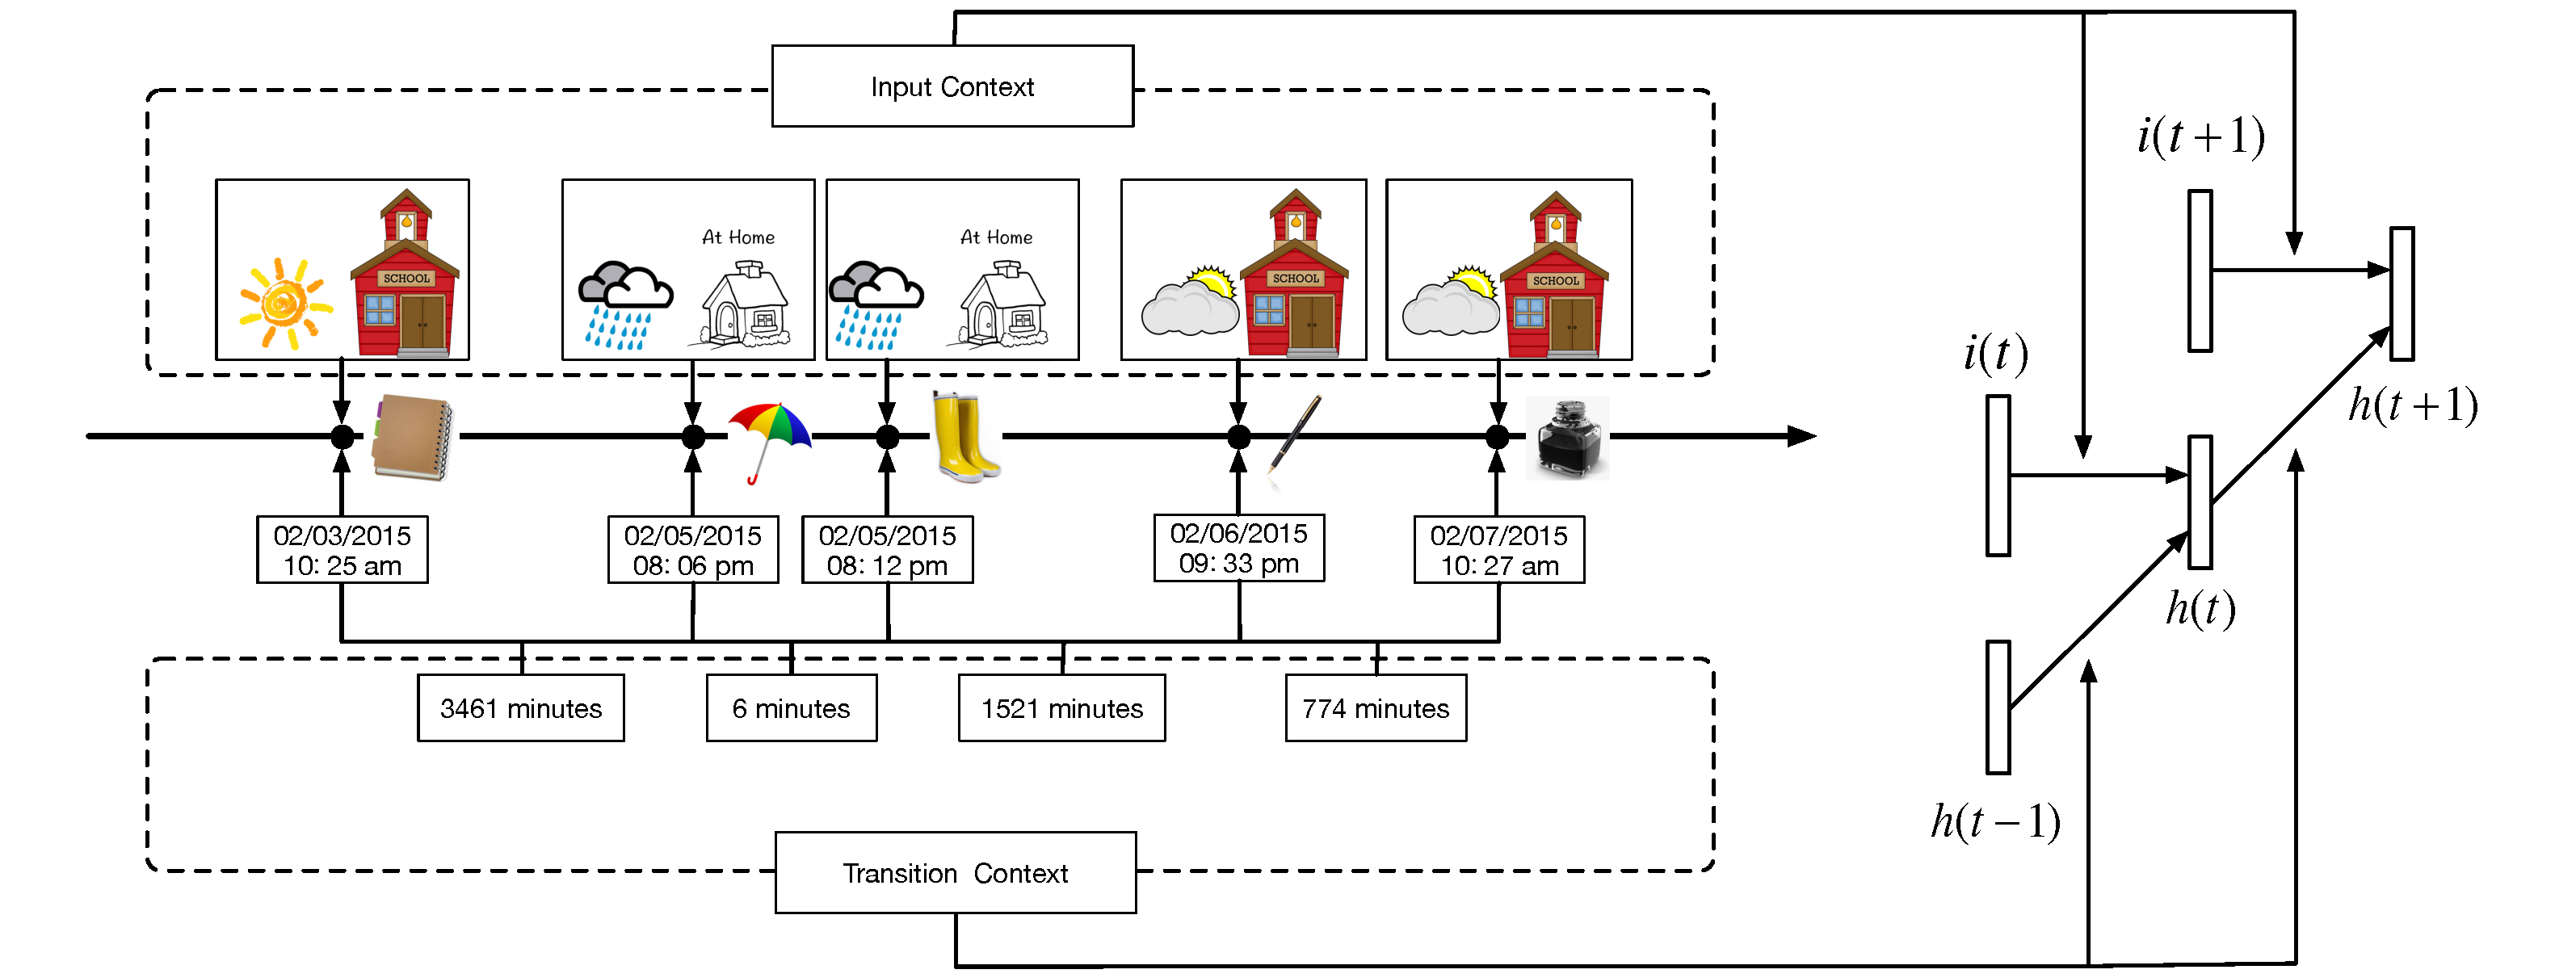
\includegraphics[width=1\linewidth]{./introModel.pdf}
\caption{The scenario of online purchase as an example of CA-RNN sequential prediction. The left part shows input contexts are situations that users conduct behaviors and transition context is time interval between adjacent behaviors in sequences. The right part illustrates how the input context and transition context are used in recurrent neural networks to predict user's next prefered item.}
\label{fig:Model-intro}
\end{figure*}

\section{Introduction}
Nowadays, people are overwhelmed by huge amount of information, the exposure to information made people tired of extracting useful and valuable information that they are interested in. This phenomenon turns out to facilitate the development of recommender systems in social networking, e-commerce, online movie and reading websites. Recommender system has now been an important tool for helping people to filter information and locate their preference. Conventional recommendation methods focus on modeling users' preference based on their historical choices of items and always ignore the sequential information. However, user preferences always change with time. Historical behaviors in different time periods have different effects on users' next choice. Accordingly, sequential recommendation is a crucial task for predicting users' next behaviors in recommender sysytems.

Nowadays, the importance of sequential information in recommender system has been gradually recognized by researchers in many disciplines, and some efforts have been put into developing CF methods with sequential information \cite{campos2014time}. Markov Chain (MC) based models \cite{yang2010personalizing,rendle2010factorizing,natarajan2013app,chen2015personalized} have been widely used for sequential prediction. MC based models aim to predict the users' next behavior based on the past behaviors in sequential data. A transition matrix is estimated, which can give the probability of an action based on the previous ones. For personalized recommendation, Factorization Personalized Markov Chain (FPMC) \cite{rendle2010factorizing} provides more accurate prediction by factorizing a personalized transition tensor. However, a major problem of MC based models is that all the components are independently combined, indicating that it makes strong independence assumption among multiple factors. Furthermore, MC based methods have been extended via representation learning, which have been applied to next basket recommendation \cite{wang2015learning}. Recently, as another typical representation learning method, Recurrent Neural Networks (RNN) have been employed to model temporal dependency for different applications successfully. RNN consists of an input layer, an output unit and multiple hidden layers. Hidden representation of RNN can change dynamically along with a sequential history. Each layer of RNN contains an input element and recurrent transition from the previous status, which are captured by an input matrix and a transition matrix respectively. RNN is famous for its being successfully applied in sentence modeling tasks \cite{mikolov2010recurrent,mikolov2011extensions,mikolov2011rnnlm}. It also achieves state-of-the-art performances in sequential click prediction \cite{zhang2014sequential}, location prediction \cite{liu2016strnn} and next basket recommendation \cite{yu2016dream}. Considering its great performances in sequential modeling tasks, RNN is a suitable tool for sequential recommendation.

Though RNN has achieved satisfactory performances, it still has its drawbacks in sequential recommendation situations. Nowadays, with enhanced ability of systems in collecting information, a great amount of contextual information in recommender systems has been collected such as location, time, weather and so on. These kinds of contextual information have significant effect on user behaviors. For instance, a man may like to watch cartoon with his children while may like to watch romantic movies with his wife. He may prefer to read novels during weekend while may tend to read professional books during weekdays. Contextual information has been proved to be useful in determining users' preferences in recommender systems \cite{palmisano2008using,adomavicius2011context}. Context-aware recommendation has been extensively studied and several methods have been proposed to achieve state-of-the-art performances \cite{rendle2011fast,shi2012tfmap,jamali2013heteromf,shi2014cars,liu2015cot}. Without considering the rich contextual information in real world, RNN and other sequential recommendation methods can only model historical sequences and are hard to further improve the performances of recommendation in complex real applications. In contrast, there are also no context-aware recommendation methods that take sequential information into consideration. Unfortunately, as shown in the example in Figure \ref{fig:Model-intro}, complex real-world applications usually have both sequential and contextual information. Thus, context-aware recommendation becomes an emerging task, and adapting RNN for variety of contextual information is a good methodology.

To incorporate contextual information in RNN and other sequential models, we investigate the properties of sequential behavioral histories and conclude two types of contexts: \textbf{input contexts} and \textbf{transition contexts}. These two types of contexts are shown in the demonstration in Figure \ref{fig:Model-intro}. And we will explain them one by one.

Input contexts denote the contexts of input elements in behavioral sequences, that is to say, input contexts are situations that users conduct behaviors, e.g., shopping, visiting or reading. Such contexts usually include location (home or working place), time (weekdays or weekends, mourning or evening), weather (sunny or rainy) and so on. As we mentioned above, input contexts have significant effects on predicting present behaviors of users. Similarly, input contexts in the history are also useful for predicting the future. For instance, if a man usually takes exercise in the morning, then we can predict he will go to the fitting room in the morning rather than evening, even if there are also lots of people going to fitting rooms in the evening.

Transition contexts are the contexts for the transition from previous behaviors in historical sequences. They capture how the previous behaviors affect the future. Specifically, transition contexts denote time intervals between adjacent behaviors in sequences in this paper. Generally speaking, longer time intervals and shorter time intervals mean different for the transition from the past. If a user's last behavior on an online shopping website happens half a year ago, then his or her past behaviors have limited effects on the user's future purchasing and a recommendation with popular items may be a better choice. If the user's last behavior happens yesterday, then his or her next purchase will be significantly affected by the previous ones and a personalized recommendation should be made.

Thus, to model sequential information and contextual information in one framework, we propose a novel model called Context-Aware Recurrent Neural Networks (\textbf{CA-RNN}). Instead of a constant input matrix for capturing input elements in each layer of RNN, we use context-specific input matrices for each specific input contexts. Similarly, we use context-specific transition matrices for modeling transition effects from previous behaviors in historical sequences under specific transition contexts, i.e., time intervals between adjacent behaviors. Then, we implement our CA-RNN model in a Bayesian Personalized Ranking (BPR) \cite{rendle2009bpr} framework to make personalized ranking of recommended items, and Back Propagation Through Time (BPTT) \cite{rumelhart1988learning} is applied for learning parameters of CA-RNN. In summary, the main contributions of this work are listed as follows:

\begin{itemize}
\item
We address the problem of context-aware sequential recommendation, which presents a novel perspective for enhanced recommendation. And we conclude two types of contexts in this problem: input contexts and transition contexts.

\item
We apply context-specific input matrices to model input contexts, which can capture the properties of contextual information in behavior histories and can make context-aware recommendations for users.

\item
We incorporate context-specific transition matrices for modeling transition contexts, i.e., time intervals between adjacent behaviors in historical sequences. This process captures transition effects from the past behaviors to the future behaviors within different time intervals.

\item
Experiments conducted on two real-world datasets show that CA-RNN is effective and clearly outperforms the state-of-the-art methods.

\end{itemize}

The rest of the paper is organized as follows. In section 2, we review some related work on sequential recommendation and context-aware recommendation. Then we give the formulation of context-aware sequential recommendation in section 3. Section 4 details our CA-RNN model. In section 5, we introduce the learning methods of our proposed model. In section 6, we conduct experiments in two real-world datasets and compare with several state-of-the-art methods. Section 7 concludes our work and discusses future research.

\section{Related Works}
In this section, we review some related works on sequential recommendation and context-aware recommendation.
%2.1
\subsection{Sequential Recommendation}

Time-aware neighbourhood models \cite{ding2005time,lathia2009temporal,liu2010online} may be the most natural methods for modeling sequences, which employ neighbourhood based algorithms to capture temporal effects via giving more relevance to recent observations and less to past observations. Using frequent pattern mining, sequential pattern based methods \cite{mobasher2002using,hariri2012context} seek sequential patterns that occur most frequently to predict the future. However, both neighbourhood based and sequential pattern based methods are unable to reveal the underlying properties in users' historical sequences. And sequential pattern based methods are time consuming in large scale datasets.

Matrix factorization based methods \cite{koren2009matrix} have become the state-of-the-art approach to conventional recommendation, which have been extended to time-aware factorization based models recently. Tensor Factorization (TF) \cite{xiong2010temporal,bahadori2014fast} treats time intervals as another dimension and generate latent vectors of time intervals via factorization to capture the underlying properties in historical sequences. TimeSVD++ \cite{koren2010collaborative} learns time-aware representations for users and items. However, factorization based models have difficulties in generating latent representations for time intervals which has never or seldom appeared in the training data.

The MC based methods are widely used models for sequential applications \cite{yang2010personalizing}. Via factorization of the probability transition matrix, Factorizing Personalized Markov Chain (FPMC) \cite{rendle2010factorizing} can provide more accurate prediction for each sequence. FPMC is also extended by using user group \cite{natarajan2013app} or incorporating location constraint \cite{cheng2013you}. Recently, some factors of human brain have been added into MC based methods, including interest-forgetting curve \cite{chen2015personalized} and dynamics of boredom \cite{kapoor2015just}. However, the main drawback of MC based models is the independent combination of the past components, which lies in a strong independence assumption and confines the prediction accuracy. MC based methods are then extended by representation learning. Hierarchical Representation Model (HRM) \cite{wang2015learning} learns the representation of behaviors in the last transaction and predicts behaviors for the next transaction. And Personalized Ranking Metric Embedding (PRME) \cite{feng2015personalized} learns embeddings of users according to the location distance.

Recently, a few prediction models, especially language models, are proposed based on neural networks. The most classical language model is proposed via a single layer neural network \cite{bengio2003neural}. And models based on RNN have been successfully used in modeling sentences \cite{mikolov2010recurrent,mikolov2011extensions,mikolov2011rnnlm}. RNN also brings satisfying results for sequential click prediction for sponsored search \cite{zhang2014sequential}, location prediction \cite{liu2016strnn} and next basket recommendation \cite{yu2016dream}. RNN is showing its great performances in sequential modeling.

%2.2
\subsection{Context-aware Recommendation}
Context-aware recommender system (CARS) \cite{adomavicius2011context} generates more relevant recommendations by adapting them to the specific contextual situation of the user, and it built based on the knowledge of contextual user preferences and typically deal with data records of user, item and context. Recent works on contextual modeling approaches extend the user-item preference relations with contextual information and incorporate factorization models to compute recommendations. Multi-verse recommendation \cite{karatzoglou2010multiverse} uses tensor factorization to model n-dimensional contextual information. The social network aided context-aware recommender system \cite{liu2013soco} splits contexts and performs general matrix factorization on each leaf of decision trees. As a extended model of tensor factorization, Factorization Machine (FM) \cite{rendle2011fast} can model a wide variety of contextual information by specifying contextual information as the input dimensions and provide context-aware predictions. The work on Heterogeneous Matrix Factorization (HeteroMF) \cite{jamali2013heteromf} generates context-specific latent vectors of entities using a context-dependent transfer matrix and the original latent vectors of entities. The Tensor Factorization for MAP maximization (TFMAP) model \cite{shi2012tfmap} uses tensor factorization and Mean Average Precision (MAP) objective to model implicit feedback data with contextual information. The newly CARS2 \cite{shi2014cars} and Contextual Operating Tensor (COT) \cite{liu2015cot} models represent the common semantic effects of contexts as contextual operating tensor and represents contexts as latent vectors. And the Hierarchical Interaction Representation (HIR) model \cite{liu2015collaborative} generates the interaction representation via tensor multiplication which can be applied in context-aware recommender system.

\section{Proposed Model}
%figure2
\begin{figure*}[htb]
\centering
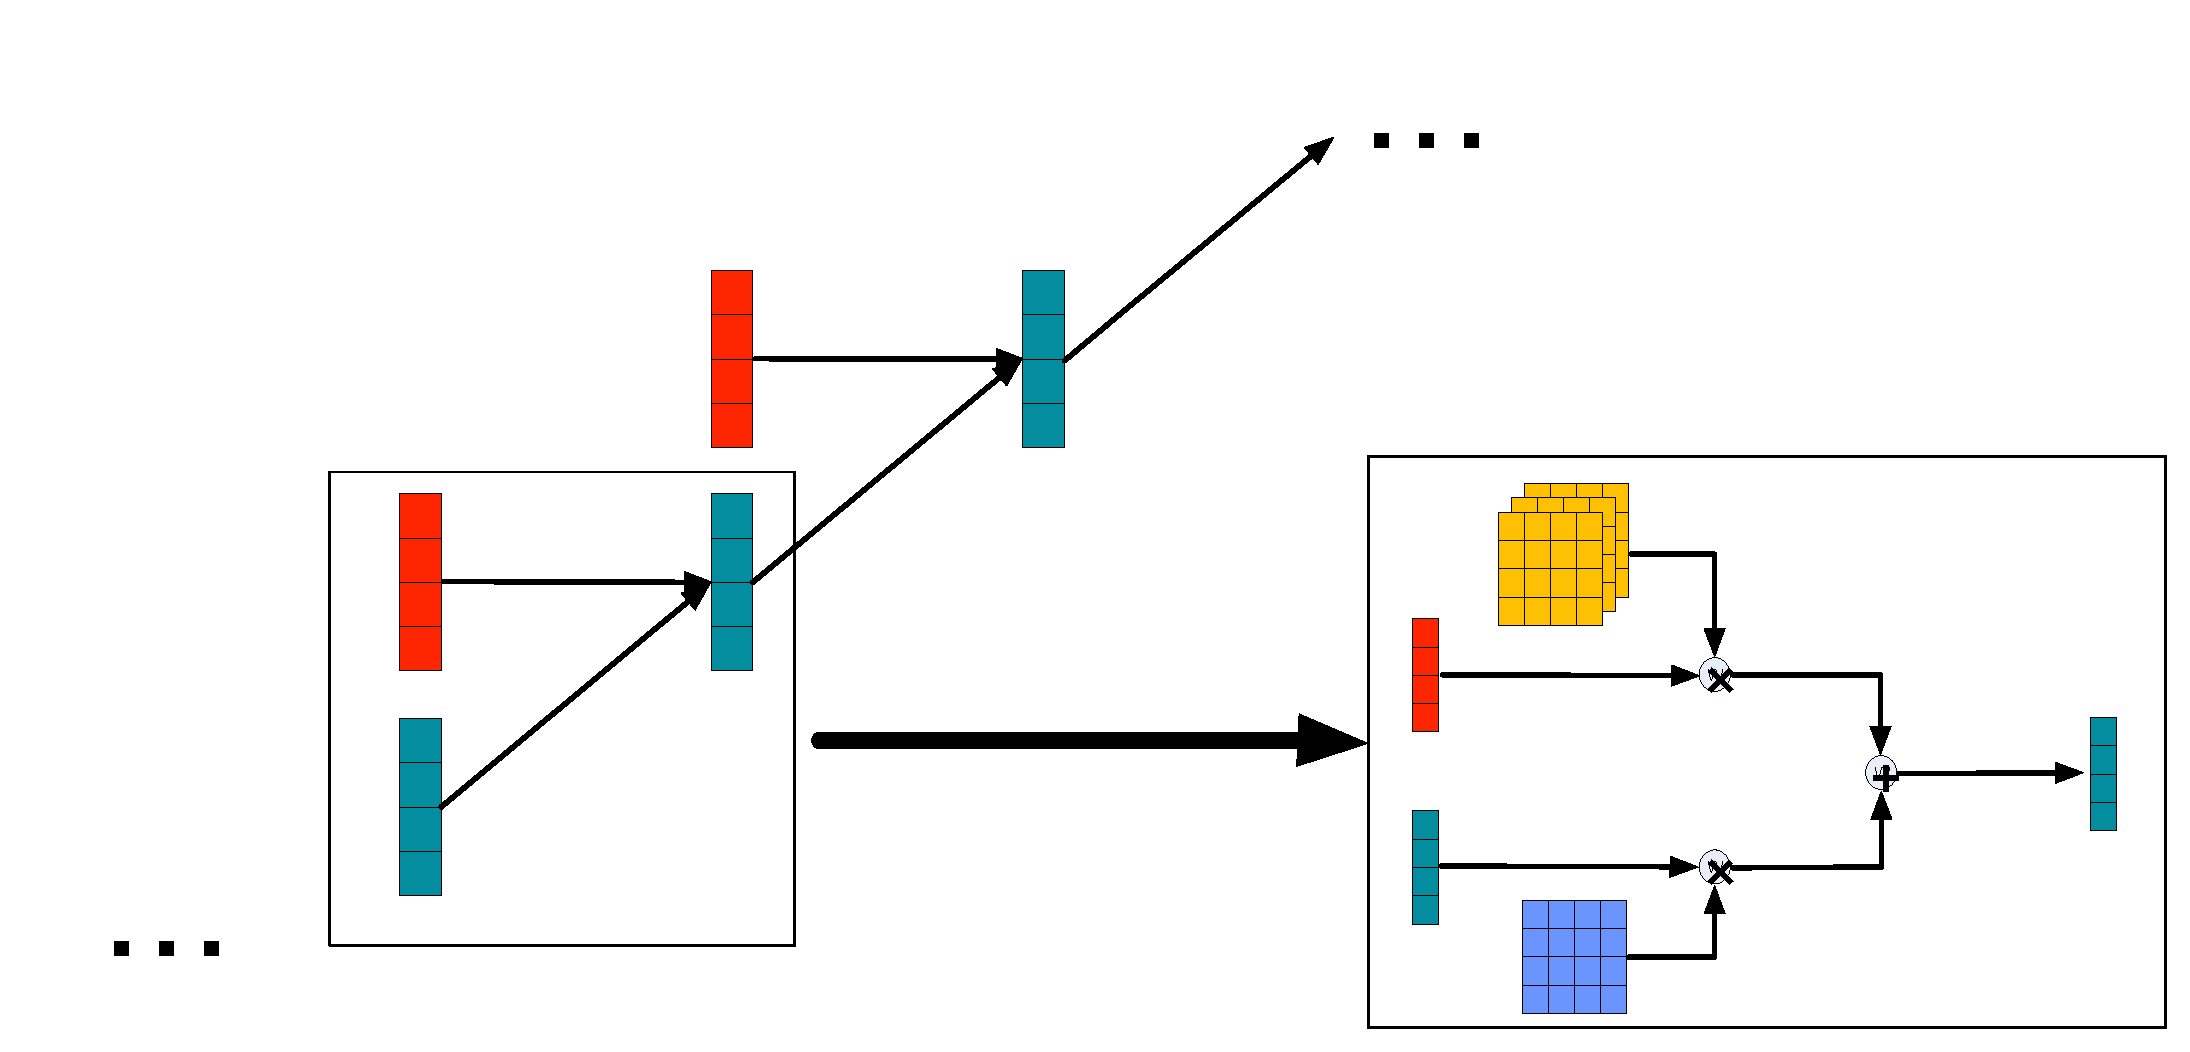
\includegraphics[width=1\linewidth]{./model.pdf}
\caption{Overview of proposed CA-RNN model. The right small square shows a state of CA-RNN. The left square illustrates the computational procedure of hidden layer in that state.}
\label{fig:Model-overview}
\end{figure*}

%3.1
\subsection{Problem Formulation}
We have a set of users denoted as $U  = \{ u_1 ,u_2 ,...\}$, a set of items denoted as $V  = \{ v_1 ,v_2 ,...\}$. There are multiple input contexts denoted as $C_I = \{C_{i1} ,C_{i2} ,...\}$, where the $C_{ik}$ denotes for one specific context such as weather, location, mood and so on. Meanwhile, each context contains several conditions. For example, mood context may consist of happy, sad and flat. The transition context $C_T$ accounts for the different time interval between two records of user. For each user $u$, the behavioral history is given as $V^u = \{v^u_{1}, v^u_{2}, ...\}$, where $v^u_{i}$ denotes the $i$ th selected item of user. And the history of all users is denoted as $V^U = \{V^u_{1}, V^u_{2}, ...\}$. The behavioral history is associated with corresponding timestamps $T^u = \{t^u_{1}, t^u_{2}, ...\}$ where $t_k$ denotes the $k$ th timestamp in one sequence. For each user $u$, at specific timestamp $t_k^u$, an combination of input contexts is denoted as $c_{I,k}^{u} = \{
c_{i1,k}^{u},c_{i2,k}^{u},...\}$ and the transition context is denoted as $c_{T,k}^{u}$ which is decided by the interval type between $t_k^u$ and $t_{k-1}^u$.






%3.2
\subsection{ Recurrent Neural Networks}
The architecture of a recurrent neural network consists of an input layer $i$, a hidden layer $h$, an output unit, as well as inner weight matrices \cite{zhang2014sequential}. RNN model the current output as the function of the previous output and a hidden layer. At each time steps, we can predict the output unit given the hidden layer, and then feed the new output back into the next hidden state. The vector representation of the hidden layer is:
\begin{equation}  \label{eqHoriginal}
\mathbf{h}_{k}^{u}=f\left ( {\mathbf{r}_{v_{k}^{u}}}\mathbf{M}+\mathbf{h}_{k-1}^{u}\mathbf{W} \right),~
\end{equation}
where $\mathbf{h}^u_{k}$ is the $d$ dimensional representation of  user $u$ at time $k$ in a behavior sequence, $\mathbf{r}_{v_{k}^{u}}$ denotes the $d$ dimensional latent vector of the corresponding item the user selects, $\mathbf{W}$ is the $d \times d$ dimensional recurrent connection of the previous status propagating sequential signals and $\mathbf{M}$ denotes the $d \times d$ dimensional transition matrix for input elements to capture the current behavior of the user. The activation function $f(x)$ is chosen as a $sigmoid$ function $f(x) = \exp \left( {1 \mathord{\left/ \right. \kern-\nulldelimiterspace} 1 + e^{ - x} } \right)$.

%3.3
\subsection{ Incorporating Transition Context}
The length of time interval between two statues has different impacts on prediction and long time interval seems to have limited effect in predicting next behavior compared with short ones. Therefore, the length of time interval is essential for predicting future behaviors. We incorporate Transition Context for time interval in the formula. The transition matrix $\textbf{W}$ is replaced with type-specific transition matrices based on transition context. Thus, Equation \ref{eqHoriginal} should be rewritten as: 
\begin{equation}  \label{eqh}
\textbf{h}_{k}^{u}=f\left ( \textbf{r}_{v_{k}^{u}}\textbf{M}+\textbf{h}_{k-1}^{u}\textbf{W}_{ t_k^u-t_{k-1}^u  }\right )~,
\end{equation}
 where $t_k^u$ and $t_{k-1}^u$ denotes the present and the previous statues respectively, $t_k^u-t_{k-1}^u$ is the time interval.  All kinds of time intervals are continuously classified into several types according to their length. We suppose that each type should contain near the same quantity of different time intervals. Then, Equation \ref{eqh} should be rewritten as: 
\begin{equation}  
\textbf{h}_{k}^{u}=f\left ( \textbf{r}_{v_{k}^{u}}\textbf{M}+\textbf{h}_{k-1}^{u}\textbf{W}_{c_{T,k}^{u}}\right )~,
\end{equation}
where $c_{T,k}^{u}$ denotes for the transition context depending on the type of the time interval between $t_k^u$ and $t_{k-1}^u$ .



%3.4
\subsection{ Context-aware Recurrent Neural Networks}
Since context information is important in future predictions and conventional RNN cannot model it, it is essential to involve context information in our model. Thus, we add the input context $c_{I,k}^{u}$ to the transition matrix $\textbf{M}$ in traditional RNN model. In CA-RNN model, given a user $u$, his or her vector representation at time $k$ can be calculated by using an integrated contextual operating matrix for a specific context combination. This matrix describe how a contexts combination affects the properties of entities and how context-specific latent vectors of users and items can be generated from their original ones. Here, we can calculate context-specific latent vectors as: 
\begin{equation}\label{eqHt}
\textbf{h}_{k}^{u}=f\left ( \textbf{r}_{v_{k}^{u}}\textbf{M}_{c_{I,k}^{u}}+\textbf{h}_{k-1}^{u}\textbf{W}_{c_{T,k}^{u}}\right )~,
\end{equation}

where  $\textbf{W}$ is a $d\times d$ dimensional transition matrix from the last status, $\textbf{r}_{v_{k}^{u}}$ is a  $d$ dimensional vector representation of the input item at time $k$ of user $u$, and $\textbf{M}_{c_{I,k}^{u}}$ is a  $d\times d$ transition matrix denotes the combination of corresponding input contexts for users and items.  

We can introduce various combination operations to model different interactions among multiple input contexts. In this work, we study three typical combination operations as follows.

\begin{itemize}
\item Linear Method: Linear computation is the most common method to calculate the combination of all contextual operating matrices, It treats the effects of each context separately, and the $\textbf{M}_{c_{I,k}^{u}}$ can be calculated as :
\begin{equation} \label{eqMadd}
\textbf{M}_{c_{I,k}^{u}} = \sum_{c_{i,k}^{u}\in C^I} \textbf{M}_{c_{i,k}^{u}} ~.
\end{equation}

\item Multiplied Method: In STRNN  \cite{liu2016strnn} ,the author incorporates temporal and spatial contexts into conventional RNN by mutipling time-specific operating matrix and distance-specific operating matrix. Analogously, we can treat input contextual operating matrices in the same way :
\begin{equation}
\textbf{M}_{c_{I,k}^{u}} = \prod_{c_{i,k}^{u}\in C^I} \textbf{M}_{c_{i,k}^{u}} ~.
\end{equation}

\item Condition-specific Method: Other than handling these input contexts matrices, the $\textbf{M}_{c_{I,k}^{u}}$ can also be a condition-specific matrix. It means that each condition has its own matrix. For example, if there are two input contexts: weather ${w_1,w_2,w_3...}$ and mood ${m_1,m_2,m_3...}$. Each parameter above accounts for a specific condition, such as $w_1$ denotes for the sunny weather and $m_1$ denotes for the happy mood. Then, there will be a matrix $M_{w_1,m_1}$ for the sunny-happy condition. In that case, the $\textbf{M}_{c_{I,k}^{u}}$ equals to such a matrix $M_{w_1,m_1}$ representing a condition under specific input contexts at time $k$. 

\end{itemize}

%3.5
\subsection{Context-aware Prediction}

Finally, the prediction of CA-RNN can be yielded via calculating inner product of user and item representations. The prediction of whether user $u$ purchase item $v$  under context $c$ at status $k+1$ can be computed as:
\begin{equation}
y_{u, k+1, c, v} = \mathbf{h}_{k}^{u}\mathbf{P}_{c, k+1}(\mathbf{r}_{v})^ \mathrm{ T }~
\end{equation}
where $\mathbf{P}_{c, k+1}$ is the representation of input context and transition context at status $k+1$. And it can be calculated by the addition or multiplication of $\mathbf{M}^{'}$ and $\mathbf{W}^{'}$ , the corresponding matrix of the two kinds context . Unlike $\mathbf{M}$ and $\mathbf{W}$ in equation 4, which are transition matrices, $\mathbf{M}^{'}$ and $\mathbf{W}^{'}$ are designed for incorporating context information to improve the predicting process. According to our experiments, addition performances better, so $\mathbf{P}_{c, k+1}$ can be calculated as:
\begin{equation}   \label{eqPadd}
\mathbf{P}_{c, k+1}=\mathbf{M}_{c_{I,k+1}^{u}}^{'} + \mathbf{W}_{c_{T,k+1}^{u}}^{'}~
\end{equation}
where $\mathbf{M}_{c_{I,k+1}^{u}}^{'}$ is the represntation of specific input contexts combination for user $u$ at time $k$ , and $\mathbf{W}_{c_{T,k+1}^{u}}^{'}$ is the represntation of transition context for interval between the current and the next status. These matrices indicate the effect of current context to the following behavior.




%3.6
\subsection{Parameter Learning}

In this subsection, we introduce the learning process of CA-RNN with Bayesian Personalized Ranking (BPR) \cite{rendle2009bpr} and Back Propagation Through Time (BPTT) \cite{rumelhart1988learning}.
BPR is a state-of-the-art pairwise ranking framework for the implicit feedback data. The basic assumption of BPR is that a user prefers a selected item than a negative one. Thus, the training objective of CA-RNN in BPR framework is to maximize the following probability:
\begin{equation}
p(u, k+1, c, v\succ v') = g(y_{u, k+1, c, v} - y_{u, k+1, c, v'}),~
\end{equation}
where $v'$ denotes a negative item sample, and $g(x)$ is a nonlinear function which is selected as $g(x) = {1 \mathord{\left/ \right. \kern-\nulldelimiterspace} 1 + e^{ - x}}$. Incorporating the negative log likelihood, we can solve the following objective function equivalently:
\begin{equation}
J = \sum \ln(1+e^{-(y_{u,k+1,c,v} - y_{u,k+1,c,v'})})+\frac{\lambda }{2}\left \| \Theta  \right \|^{2}  ~,
\end{equation}
where $\lambda = {R, M ,W}$ denotes all the parameters to be estimated, $\lambda$ is a parameter to control the power of regularization. And the derivation of $J$ with respect to the parameters can be calculated as: 
\begin{displaymath}
\frac{\partial J}{\partial \mathbf{r}_{v}} = -\sum \frac{\mathbf{h}_{k}^{u}\mathbf{P}_{c,k+1}e^{-(y_{u, k+1, c, v} - y_{u, k+1, c, v'})}}{1+e^{-(y_{u, k+1, c, v} - y_{u, k+1, c, v'})}}+\lambda \mathbf{r}_{v}  ~,
\end{displaymath}
\begin{displaymath}
\frac{\partial J}{\partial \mathbf{r}_{v'}} = \sum \frac{\mathbf{h}_{k}^{u}\mathbf{P}_{c,k+1}e^{-(y_{u, k+1, c, v} - y_{u, k+1, c, v'})}}{1+e^{-(y_{u, k+1, c, v} - y_{u, k+1, c, v'})}}+\lambda \mathbf{r}_{v'}  ~,
\end{displaymath}
\begin{displaymath}
\frac{\partial J}{\partial \mathbf{h}_{k}^{u}} = -\sum \frac{(\mathbf{r}_{v}-\mathbf{r}_{v}^{'})(\mathbf{P}_{c,k+1})^{\mathrm{ T }}e^{-(y_{u, k+1, c, v} - y_{u, k+1, c, v'})}}{1+e^{-(y_{u, k+1, c, v} - y_{u, k+1, c, v'})}}   ~,
\end{displaymath}
\begin{displaymath}
\frac{\partial J}{\partial \mathbf{P}_{c,k+1}} = -\sum \frac{(\mathbf{h}_{k}^{u})^{\mathrm T}(\mathbf{r}_{v}-\mathbf{r}_{v}^{'})e^{-(y_{u, k+1, c, v} - y_{u, k+1, c, v'})}
}{e^{-(y_{u, k+1, c, v} - y_{u, k+1, c, v'})}}    ~.
\end{displaymath}

Moreover, parameters in CA-RNN can be further learnt with the BPTT algorithm. According to Equation \ref{eqHt}, given the derivation ${\partial J \mathord{\left/ \right. \kern-\nulldelimiterspace} {\partial \mathbf{h}_{k}^{u} } }$, the corresponding gradients of all parameters in the hidden layer can be calculated as: 
\begin{displaymath}
\frac{{\partial J}}{{\partial \mathbf{h}^u_{k-1} }} =  \left( {f'\left(  \cdot  \right) \otimes \frac{{\partial J}}{{\partial \mathbf{h}^u_{k} }}} \right)\left({\mathbf{W}_{c_{T,k}^{u}}}\right)^\mathrm{T} ~,
\end{displaymath}

\begin{displaymath}
\frac{{\partial J}}{{\partial {\mathbf{W}_{c_{T,k}^{u}}} }} =  \left({\mathbf{h}_{k-1}^u}\right)^\mathrm{T}\left( {f'\left(  \cdot  \right) \otimes \frac{{\partial J}}{{\partial \mathbf{h}^u_{k} }}} \right) ~,
\end{displaymath}

\begin{displaymath}
\frac{{\partial J}}{{\partial \mathbf{r}_{v_k^u} }} =  \left( {f'\left(  \cdot  \right) \otimes \frac{{\partial J}}{{\partial \mathbf{h}^u_{k} }}} \right)\left({\mathbf{M}_{c^u_{I,k+1}}}\right)^\mathrm{T} ~,
\end{displaymath}

\begin{displaymath}
\frac{{\partial J}}{{\partial {\mathbf{M}_{c^u_{I,k+1}}} }} =  \left({\mathbf{r}_{v^u_k}}\right)^\mathrm{T}\left( {f'\left(  \cdot  \right) \otimes \frac{{\partial J}}{{\partial \mathbf{h}^u_{k} }}} \right) ~.
\end{displaymath}
This process can be repeated iteratively in the whole behavioral sequence. 
Then, according to Equation \ref{eqMadd} and \ref{eqPadd}, given ${\partial J \mathord{\left/ \right. \kern-\nulldelimiterspace} {\partial \mathbf{P}_{c,k+1} } }$, the gradients of $\mathbf{M}^{'}_{c^u_{i,k+1}}$, $\mathbf{M}_{c^u_{i,k+1}}$ and $\mathbf{W}^{'}_{c_{T,k+1}^{u}}$ can be computed as: 
\begin{displaymath}
\frac{{\partial J}}{{\partial {\mathbf{M}^{'}_{c^u_{I,k+1}}} }} =  \frac{\partial J}{\partial \mathbf{P}_{c,k+1}} ~,
\end{displaymath}
\begin{displaymath}
\frac{{\partial J}}{{\partial {\mathbf{W}^{'}_{c_{T,k+1}^{u}}} }} =  \frac{\partial J}{\partial \mathbf{P}_{c,k+1}} ~,
\end{displaymath}
\begin{displaymath}
\frac{{\partial J}}{{\partial {\mathbf{M}^{'}_{c^u_{i,k+1}}} }} =  \frac{\partial J}{\partial \mathbf{M}^{'}_{c^u_{I,k+1}}} ~.
\end{displaymath}
\begin{displaymath}
\frac{{\partial J}}{{\partial {\mathbf{M}_{c^u_{i,k+1}}} }} =  \frac{\partial J}{\partial \mathbf{M}_{c^u_{I,k+1}}} ~.
\end{displaymath}
Now, after calculating all the gradients, we can employ stochastic gradient descent to estimate the model parameters. 

\section{Experiments}
In this section, we conduct empirical experiments to demonstrate the effectiveness of CA-RNN on sequential recommendation. First we introduce the datasets, baseline methods and evaluation metrics of our experiments. Then we compared our CA-RNN to the state-of-the-art methods. Finally, we analyse the impact of parameters, especially the length of hidden layer.
\subsection{Experiment Datasets}
Our experiments are conducted on two real datasets with various contexts:
\begin{itemize}
\item \textbf{Fashion}\footnote{https://tianchi.shuju.aliyun.com/competition/index.htm} is a public online e-commerce dataset released by TIANCHI\footnote{https://tianchi.shuju.aliyun.com/}, which records clothes purchase behaviors. It contains 13, 611, 038 records belonging to 1, 103, 702 users and 462, 008 items. The time information is collected based on the day level.

\item \textbf{Tmall}\footnote{https://102.alibaba.com/competition/addDiscovery/index.htm} is a public dataset from Tmall\footnote{https://www.tmall.com/}, one of the biggest online shopping websites in China. It covers products from food, clothes to electrical appliance and records the online transactions in terms of brands. It contains 182, 881 records belonging to 885 users and 9, 532 brands.The temporal information in the dataset is extracted based on day level.
\end{itemize}

We conduct some pre-process on these transaction datasets. For Fashion dataset, firstly we remove all the users that have bought in total less than 10 items. Second, we iteratively remove items bought by less than 3 times and users who have purchased the removed items. The second step is to make sure that each item is bought greater than or equal to 3 times and the transition in each user's purchase sequence is not changed. For Tmall dataset, xxxxxx.

For each purchase sequence of the two datasets, we use first 90\% of the items in the sequence for training, the remaining 10\% data for testing. 


\subsection{Incorporated Contexts }
As mentioned above, we proposed to make use of two kinds of contexts named transition context and input context.

The transition context matrix $\textbf{W}_{c_{T,k}^{u}}$ is determined by the type of time interval between $t_k^u$ and $t_{k-1}^u$. The time interval is continuously classified with the prerequisite that number of records is balanced in each type, as shown in Figure \ref{fig:comparision}. Such division of time interval is reasonable because on one hand short time interval is divided carefully and long time interval is treated as similar, on the other hand the balanced number of records can ensure the effective training process.
\begin{figure}[!tb]
\centering
\subfigure[Fashion dataset.]{
\begin{minipage}[b]{0.4\textwidth}
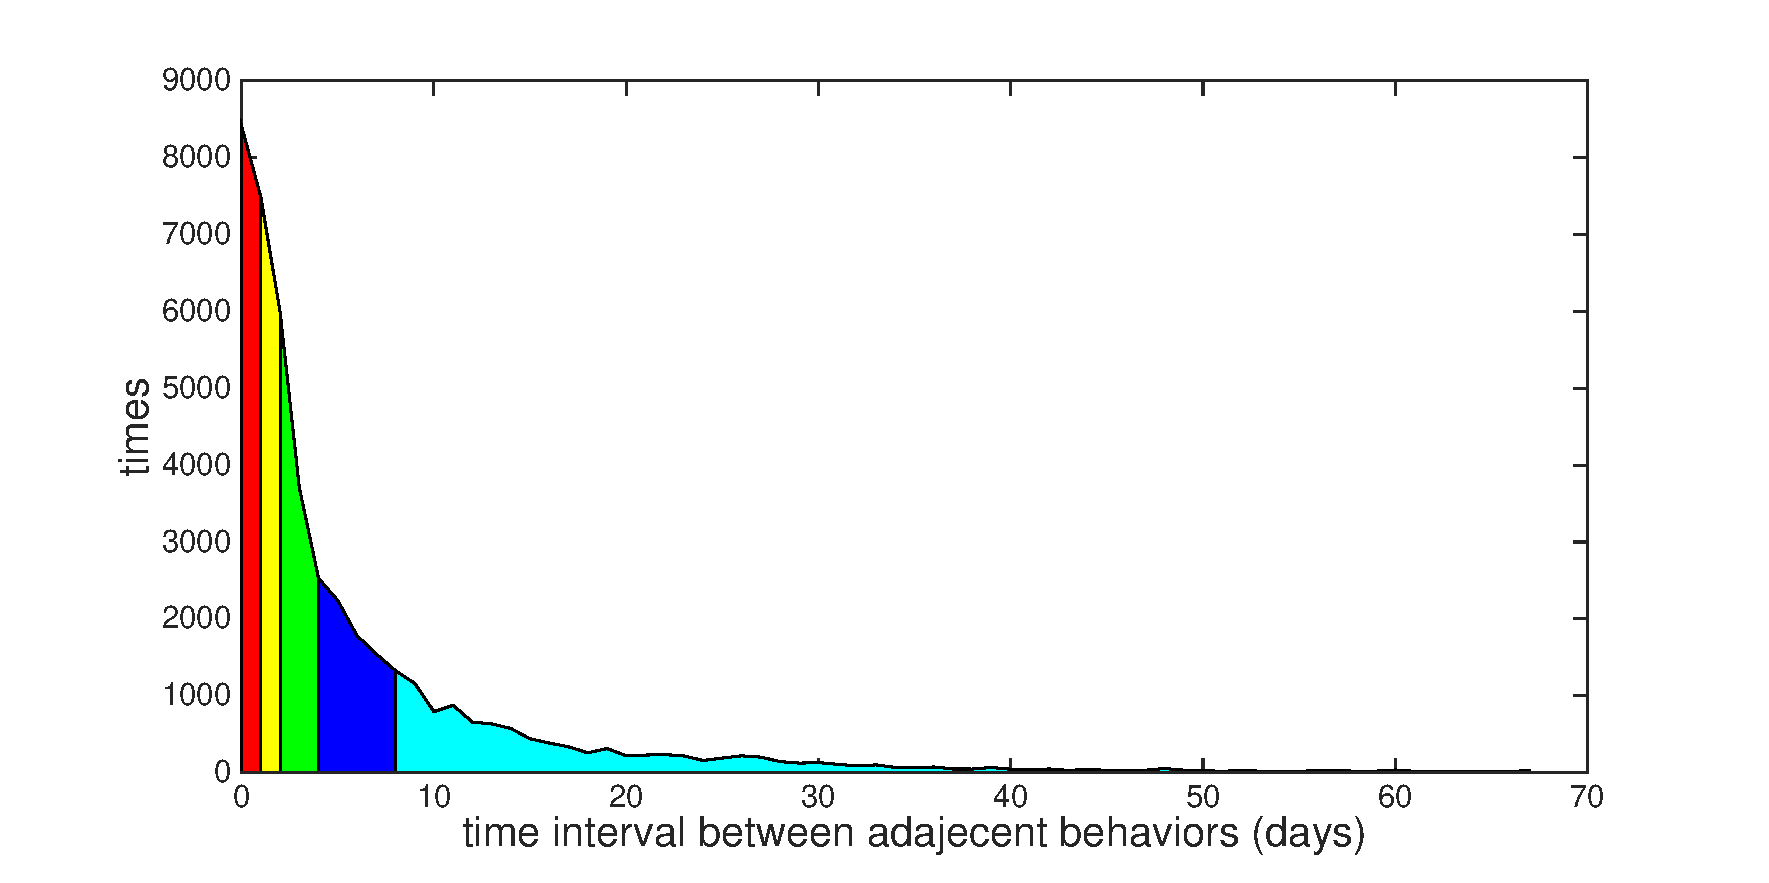
\includegraphics[width=1\textwidth]{./TimeInterval1.eps}
\label{fashion_interval}
\end{minipage}
}
\hspace{-1mm}
\subfigure[Tmall dataset.]{
\begin{minipage}[b]{0.4\textwidth}
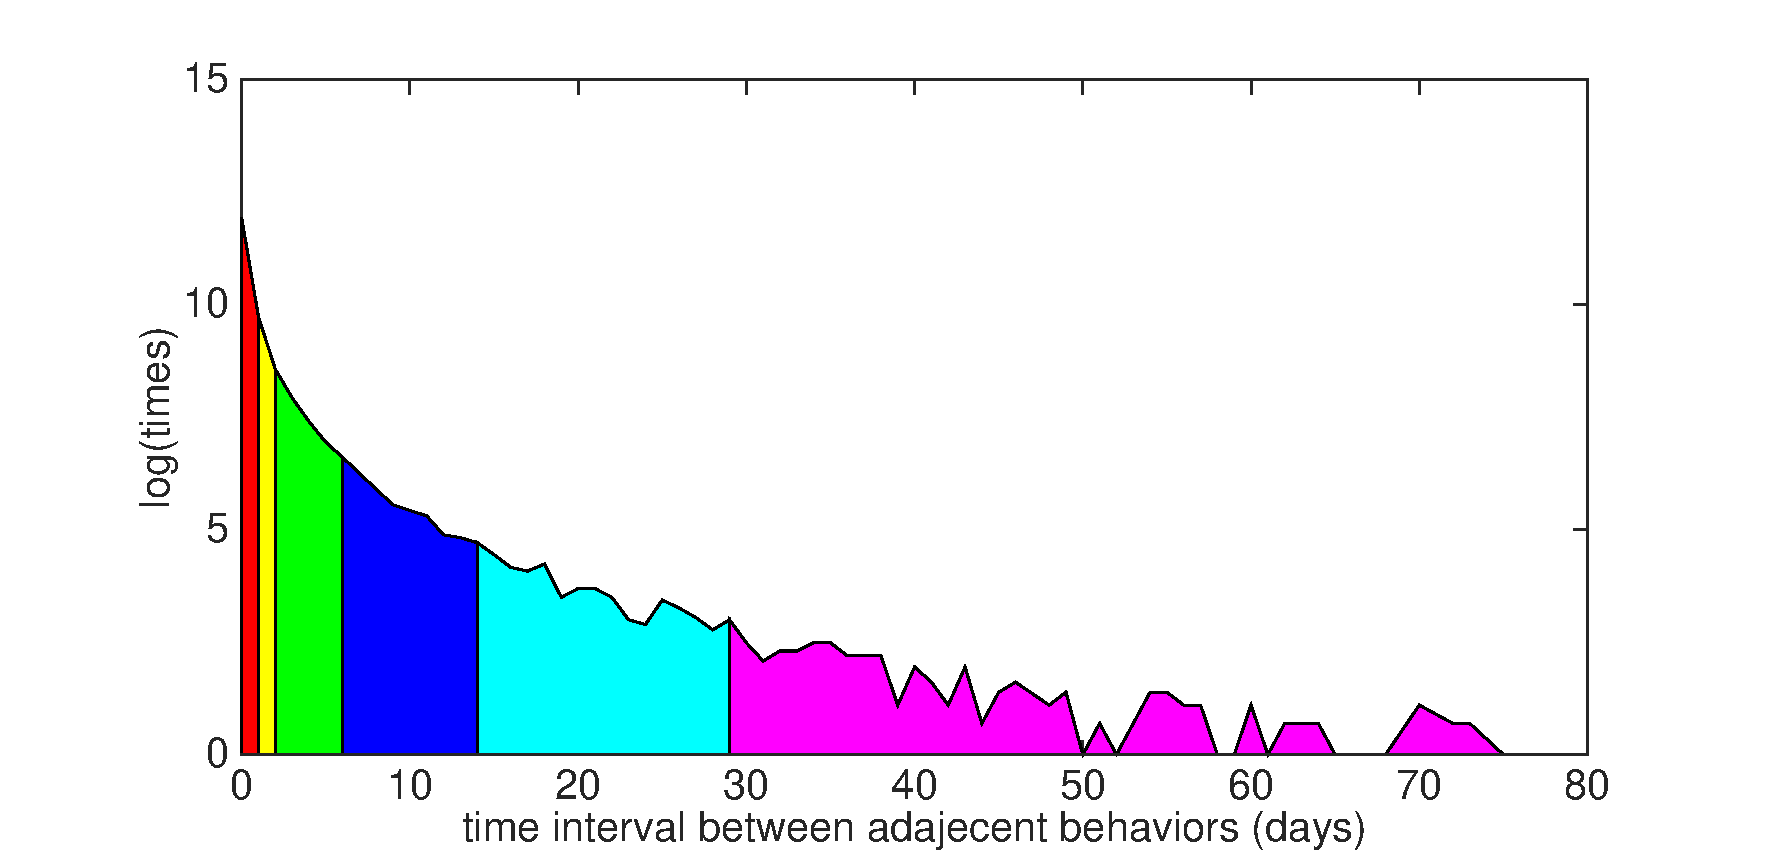
\includegraphics[width=1\textwidth]{./TimeInterval2.eps}
\label{tmall_interval}
\end{minipage}
}
\caption{Division of Time Interval.}
\label{fig:comparision}
\end{figure}

The input context consists of week context and month context. Week context represents the day of a transaction in week and month context represents that the time of a transaction is in the first, second, or the third ten-day periods of a month. These contexts have significant effects on user's next purchase behavior because people will tend to buy similar items in the beginning of the month when receiving salary and a large amount of household items are usually bought on weekend.


\subsection{Evaluation Metrics}
The output of our model is a ranked list in which items are ranked according to the value representing the preference of each user. Thus, we evaluate the performance of each method through several widely-used metrics for ranking tasks.
\begin{itemize}
\item \textbf{Recall@k} and \textbf{F1-score@k} are two important metrics for ranking tasks. The evaluation score for our experiments is computed according to the value of each user's prefered item. We report recall@k and F1-score@k with $k=1$, $5$ and $10$ in our experiments. The larger the value, the better the performance.

\item \textbf{Mean Average Precision (MAP)} is another commonly used global evaluation in ranking tasks. MAP is a standard meetric for measuring the quality of the whole ranking list. Top-bias property of MAP is particularly significant in evaluating ranking tasks such as top-N recommendation. The larger the value, the better the performance.
\end{itemize}

%table1
\begin{table*}[!htbp]
\centering\scriptsize
\caption{Performance of different method of computing the aggregation}
    \begin{tabular}{ccccccccc}
    \toprule
          & Method& recall@1 & recall@5 & recall@10&F1-score@1 & F1-score@5 & F1-score@10&MAP\\
    \midrule
    \multirow{5}[0]{*}{Tmall} 
        &Week& 0.1681& 0.3788& 0.4984& 0.1681& 0.1263& 0.0906&0.2793\\
        &Month& 0.1732& 0.3688& 0.4878& 0.1732& 0.1229& 0.0887&0.2752\\
        &Plus& \textbf{0.1748}& \textbf{0.4266}& \textbf{0.5515}& \textbf{0.1748}& \textbf{0.1422}& \textbf{0.1003}& \textbf{0.2986}\\
        &Mutiply& 0.1713& 0.4068& 0.5222& 0.1713& 0.1356& 0.0950&0.2901\\
        &Combination& 0.1765& 0.3934& 0.5068& 0.1765& 0.1312& 0.0921&0.2865\\
    \midrule
    \multirow{5}[0]{*}{Fashion} 
        &Week& 0.1087& 0.3325& 0.4713& 0.1087& 0.1108& 0.0857&0.2237\\
        &Month& 0.0839& 0.2793& 0.4125& 0.0839& 0.0931& 0.0750&0.1858\\
        &Plus& \textbf{0.1324}& \textbf{0.3720}& \textbf{0.5281}& \textbf{0.1324}& \textbf{0.1240}& \textbf{0.0960}& \textbf{0.2556}\\
        &Mutiply& 0.1157& 0.3155& 0.4861& 0.1157& 0.1052& 0.0884&0.2298\\
        &Combination& 0.1206& 0.3376& 0.4914& 0.1206& 0.1125& 0.0893&0.2346\\
    \bottomrule
\end{tabular}%
\end{table*}%

\begin{table*}[htbp]
\centering\scriptsize
\caption{Input and Transition}
\begin{tabular}{ccccccccc}
    \toprule
          &  & recall@1 & recall@5 & recall@10 & F1-score@1 & F1-score@5 & F1-score@10 & MAP   \\
    \midrule
    \multirow{3}[0]{*}{Tmall} 
        &Input   &0.1748 &0.4266 & 0.5515  &0.1748  &0.1422  &0.1003  &0.2986   \\
        &Transition  &0.1887 & 0.4134  &0.5158&  0.1887& 0.1378  &0.0938&  0.3020   \\
        &All &0.2028  &0.4171  &0.5216  &0.2028  &0.1390  &0.0948 & 0.3074\\
    \midrule
    \multirow{3}[0]{*}{Fashion} 
        &Input   &0.1324  &0.3720  &0.5281  &0.1324  &0.1240 & 0.0960  &0.2556   \\
        &Transition  &0.1129  &0.3284  &0.4392  &0.1129  &0.1095  &0.0799  &0.2186   \\
        &All &0.1648  &0.4305  &0.5804  &0.1648 & 0.1435&  0.1055  &0.2932\\
    \bottomrule
\end{tabular}%
\label{tab:InputAndTransition}%
\end{table*}%

\subsection{Compared Methods}
\begin{itemize}
\item \textbf{Top}: 
The most frequently bought items are selected as prediction for each user.
\item \textbf{MF}: 
The state-of-the-art method of collaborative filtering, analyzes relationships between users and interdependencies among items.
\item \textbf{FM}: 
FMs are easily applicable to a wide variety of contexts. It has a linear complexity and empirically provide a better prediction quality in much less time.
\item \textbf{CARS2}: 
Utilizing an appropriate model that aims to represent the type of interactions between context variables, users and items.
\item \textbf{FPMC}: 
A method brings matrix factorization (MF) and Markov chains (MC) together. It can capture
both sequential effects and long term user-taste.
\item \textbf{HRM}: 
It utilizies both sequential behavior and users$'$ general taste by involving transaction and user representations in prediction. Applying different aggregation operations to model complicated interactions among different factors.
\item \textbf{RNN}: 
Typical method for temporal prediction, which was originally applied in word embedding. It has been successfully extended to sequential modeling. 


\end{itemize}
 To find out the best method among different aggregation operations, we aggregate the combination through Plus, Multiply and Condition-specific method respectively. Meanwhile, in order to discuss the individual effect of input contexts and transition context, we incorporate each context to our model separately on both data set. 




\subsection{Analysis of Contexts}
As mentioned above, there are several methods, such as Plus, Multiply and Combination-specific, to compute the aggregation matrix for all contextual operating matrices. Here in this part, we will discuss the effect of each method.

As indicated in Table 1, no matter in which method, the model aggregates input contexts outperforms the model incorporating each input context respectively. On all evalution matrics, the Plus method is clearly the best one of integrating input contexts. Especially on Fashion dataset, compared with utilizing week information only, the Plus method improves the MAP value by 6.98\%. The performance of Combination-specific method seems to be close to that of the Plus method. However, the amount of parameters of Combination-specific method is larger than Plus method, this shortcut will get worse when the amount of conditions in each context is large. 

Thus, we suppose to utilize Plus method to compute the aggregation matrix for all contextual operating matrices in CA-RNN.

As discussed in the section of CARNN model, we suppose to utilize both Input context and Transition contexts simultaneously. Table 2  illustrates the comparision among incorporating different contexts seperately and put them together. The result indicates that CARNN consists of both Input and Transition contexts works on Tmall and Fashion dataset. 


\subsection{Performance Comparison}
The performance comparsion on the Tmall dataset and the Fashion dataset evaluated by recall, F1-score and MAP is illustrated in table \ref{tab:result}. Compared to the baseline performance of POP, MF, FM and CARS2 have similar performance improvement on the two datasets. Jointly modeling sequential information and collaborative information, FPMC and HRM achieve great improvement by combining both sequential behavior and users’ general taste. Learning latent representations of recent behaviors, HRM further improves the performance of FPMC. Another great improvement is brought by RNN, and it is the best one among the compared methods. Moreover, we can observe that, our proposed CARNN achieve the best performance on the Tmall dataset and the Fashion dataset in terms of all the metrics. Using the best scores of each method, comparing with RNN, the MAP improvements of CARNN are 6.74\% and 11.04\% on Tmall and Fashion respectively. These great improvements indicate the superiority of our method brought by modeling sequential information and contextual information.


\begin{table*}[htbp]
\centering\scriptsize
\caption{Performance comparison on two datasets evaluated by recall, F1-score, MAP.}
\begin{tabular}{ccccccccc}
    \toprule
          &       & recall@1 & recall@5 & recall@10 & F1-score@1 & F1-score@5 & F1-score@10 & MAP   \\
    \midrule
    \multirow{8}[0]{*}{Tmall} 
        & POP   &0.0169    &0.0944  &0.1938  &0.0169  &0.0315  &0.0352  &0.0763 \\
        & MF    &0.0425   & 0.1436  &0.2798&  0.0425  &0.0479 & 0.0509  &0.1218 \\
        & FM   &0.0584  &0.1641  &0.3018 & 0.0584  &0.0547 & 0.0549 & 0.1448 \\
        & CARS2   &0.0616 & 0.1697  &0.3106 & 0.0616 & 0.0566 & 0.0565 & 0.1496\\
        & FPMC    &0.0866  &0.2253  &0.3405  &0.0866  &0.0751  &0.0619  &0.1811 \\
        & HRM   &0.0956  &0.2488 & 0.3703 & 0.0956 & 0.0829&  0.0673&  0.2001 \\
        & RNN   &0.1282  &0.3412&  0.4392&  0.1282 & 0.1138 &0.0798 & 0.2400 \\
        & CARNN    &\textbf{0.2028}  &\textbf{0.4171}  &\textbf{0.5216}&  \textbf{0.2028}&  \textbf{0.1390}&\textbf{ 0.0948}  &\textbf{0.3074} \\
    \midrule
    \multirow{8}[0]{*}{Fashion} 
        & POP   &0.0024  &0.0246  & 0.0272  & 0.0024   &0.0082  & 0.0049   &0.0314 \\
        & MF    & 0.0145  & 0.0462  & 0.0783  &0.0145   &0.0154   &0.0142   &0.0510 \\
        & FM   & 0.0241  &0.0660  & 0.1070   &0.0241   &0.0220  & 0.0195  & 0.0732 \\
        & CARS2   &0.0257   &0.0687  & 0.1107   &0.0257  & 0.0229   &0.0201  & 0.0761 \\
        & FPMC    & 0.0581  & 0.1869  & 0.2776  & 0.0581   &0.0623  & 0.0505  & 0.1261 \\
        & HRM   & 0.0629   &0.2024   &0.2969 &  0.0629 &  0.0675 &  0.0540   &0.1366 \\
        & RNN   & 0.0859   &0.2696 &  0.3849  & 0.0859  & 0.0899 &  0.0700   &0.1828 \\
        & CARNN    & \textbf{0.1648}   &\textbf{0.4305}  &\textbf{ 0.5804}   &\textbf{0.1648}   &\textbf{0.1435} &  \textbf{0.1055 }& \textbf{ 0.2932} \\
    \bottomrule
\end{tabular}%
\label{tab:result}%
\end{table*}%



\subsection{Impact of Parameters}

Performance of CARNN, RNN, RNN with input context, RNN with transition context on Tmall dataset and Fashion dataset with varying dimensionality is shown in Figure \ref{fig:dimension}. As shown in Figure \ref{fig:dimension} (a), for Tmall dataset RNN with context achieve better performance than conventional RNN consistently with all dimensions. And even not with the best dimensionality, our methods can still outperform RNN. RNN with input context performs better than CARNN when evaluated by Recall@5 while CARNN performs best when evaluated by MAP. For Fashion dataset, the curves in Figure \ref{fig:dimension} (b) show the great advantages of CARNN comparing with other compared methods with different dimensionality evaluated by different metrics. And with increasing dimension, the value of Recall@5 and MAP incraese at first, then decrease after $d = 20$, which means that 20 is the best parameter for CARNN on Fashion dataset. We can also observe that the impact of dimensionality for Tmall dataset is smaller than that for Fashion dataset.


\begin{figure}[!tb]
\centering
{
\begin{minipage}[b]{0.5\textwidth}
\includegraphics[width=1\textwidth]{./dimension.eps}
\label{dimension}
\end{minipage}
}

\caption{Performance comparison of CARNN among RNN, RNN with input context and RNN with transition context over two datasets. The dimensionality is increased from 5 to 15 on Tmall and 5 to 40 on Fashion.}
\label{fig:dimension}
\end{figure}


% \begin{table*}[htbp]
% \centering\scriptsize
% \caption{Dimension}
% \begin{tabular}{ccccccccccccc}
%     \toprule
%         &      &5   &6   &7  & 8  & 9  & 10&  11&  12 & 13&  14  &15  \\
%     \midrule
%     \multirow{4}[0]{*}{Recall1}
%         & RNN& 0.1168  &0.1224 & 0.1246&  0.1283 & 0.1281 & 0.1278 & 0.1276&  0.1271 & 0.1267 & 0.1260 & 0.1257   \\
%         &Input   &0.1582 & 0.1689 & 0.1692  &0.1774  &0.1749  &0.1748 & 0.1755 &0.1713  &0.1715  &0.1703  &0.1680   \\
%         &Transition & 0.1740 & 0.1831&  0.1870  &0.1915 & 0.1887  &0.1887  &0.1893  &0.1871&  0.1866  &0.1840  &0.1806   \\
%         &All &0.1898  &0.1992  &0.2000  &0.2041  &0.2018 & 0.2028  &0.2002  &0.2003  &0.1983 & 0.1984  &0.1962   \\
%     \midrule
%     \multirow{4}[0]{*}{Recall5}
%         &RNN& 0.3227  &0.3343 & 0.3372 &0.3410  &0.3406&  0.3406&  0.3403 & 0.3397  &0.3391  &0.3387&  0.3381   \\
%         & Input  & 0.4043 & 0.4152&  0.4187  &0.4249&  0.4285  &0.4266  &0.4250  &0.4231  &0.4186 & 0.4181  &0.4145   \\
%         & Transition & 0.3860 &0.4000  &0.4056 & 0.4098  &0.4135  &0.4134  &0.4111&  0.4106  &0.4054  &0.3970 & 0.3899   \\
%         &All &0.3899 & 0.4057  &0.4137  &0.4181  &0.4172  &0.4171  &0.4163  &0.4149  &0.4126  &0.4096 & 0.4073   \\
%     \midrule
%     \multirow{4}[0]{*}{Recall10}
%         &RNN &0.4220&  0.4324  &0.4358 & 0.4397  &0.4393  &0.4392  &0.4388  &0.4383  &0.4376  &0.4373  &0.4368   \\
%         &Input   &0.5182  &0.5364 & 0.5440  &0.5539  &0.5532  &0.5515 & 0.5482 & 0.5448  &0.5397  &0.5364  &0.5330   \\
%         &Transition  &0.4945&  0.5077  &0.5117 & 0.5163  &0.5160  &0.5158  &0.5153  &0.5149 & 0.5138  &0.5136 & 0.5130   \\
%         &All &0.4951 & 0.5104  &0.5160  &0.5230 & 0.5225&  0.5216  &0.5198  &0.5180&  0.5150 &0.5133  &0.5114   \\
%     \midrule
%     \multirow{4}[0]{*}{MAP}
%         &RNN& 0.2284  &0.2337 & 0.2390 & 0.2413  &0.2409  &0.2400 & 0.2390&  0.2383&  0.2371  &0.2369  &0.2366   \\
%         & Input&   0.2814  &0.2896&  0.2944 & 0.2969 & 0.2994&  0.2986  &0.2963 & 0.2921&  0.2899 & 0.2863 & 0.2857   \\
%         & Transition & 0.2838  &0.2959  &0.2985  &0.3010  &0.3023  &0.3020  &0.3006 & 0.2951&  0.2913  &0.2900  &0.2881   \\
%         &  All &0.2946  &0.2972  &0.3079 & 0.3098  &0.3084  &0.3074  &0.3056 & 0.3048&  0.3029&  0.2998 & 0.2969   \\
%     \bottomrule
% \end{tabular}%
% \label{tab:Dimension1}%
% \end{table*}%

% \begin{table}[htbp]
% \centering\scriptsize
% \caption{Dimension}
% \begin{tabular}{ccccccc}
%     \toprule
%         &      &5   &10   &20  & 30  & 40 \\
%     \midrule
%     \multirow{4}[0]{*}{Recall1}
%         & RNN& 0.0443  & 0.0859 & 0.1136 & 0.1370&  0.1449 \\
%         &Input   &0.0780   &  0.1324  & 0.1334&   0.1530&   0.1501 \\
%         &Transition &   0.0729 & 0.1129&  0.1248 & 0.1185  &0.1147  \\
%         &All &0.1056  &  0.1648  &0.2082  &0.1966&  0.1707 \\
%     \midrule
%     \multirow{4}[0]{*}{Recall5}
%         &RNN&    0.1488 &   0.2696 & 0.3156&  0.3544&  0.3590\\
%         & Input  &   0.2810&  0.3720  &0.3733 & 0.4132  &0.3963 \\
%         & Transition &  0.2663 &  0.3284 & 0.3532 & 0.3418&  0.3389 \\
%         &All &0.2905  &  0.4305&  0.4947  &0.4544&  0.4430 \\
%     \midrule
%     \multirow{4}[0]{*}{Recall10}
%         &RNN & 0.2330    &0.3849  &0.4386&  0.4822&  0.4893 \\
%         &Input   &0.4270  &  0.5281&  0.5449 & 0.5818  &0.5605 \\
%         &Transition  & 0.3823 &   0.4392  & 0.4872  & 0.4656  & 0.4573 \\
%         &All & 0.4347   &0.5804 & 0.6363 & 0.6105  &0.5910 \\
%     \midrule
%     \multirow{4}[0]{*}{MAP}
%         &RNN&  0.1104  &0.1828  &0.2192 & 0.2464 & 0.2483 \\
%         & Input&  0.1848   &  0.2556  &0.2553&  0.2854&  0.2751  \\
%         & Transition &  0.1726&   0.2267  &0.2403 & 0.2357&  0.2312 \\
%         &  All & 0.2067   &0.2932&  0.3454&  0.3216&  0.3018 \\
%     \bottomrule
% \end{tabular}%
% \label{tab:Dimension2}%
% \end{table}%







\section{Conclusions and Future Work}

In this paper, we have address the problem of context-aware sequential recommendation and proposed a novel method, i.e., context-aware recurrent neural networks. In CA-RNN, the constant input matrix of conventional RNN is replaced with context-specific input matrices to modeling complex real-world contexts, e.g., time, location and weather. Meanwhile, to model transition contexts, i.e., time intervals between adjacent behaviors in historical sequences, contexts-specific transition matrices are incorporated, instead of the constant one in conventional RNN. Then, to make personalized ranking of recommended items, we implement CA-RNN in the BPR framework and apply BPTT to learn parameters in CA-RNN. The experimental results on two real datasets show that CA-RNN outperforms the state-of-the-art sequential and context-aware recommendation models.

In the future, we can further investigate the following direction. In CA-RNN, parameters are the same for different users, which does not confirm to practical situations. So, to make better personalized recommendation,+ we need to find a method to determine different parameters for different users or different user groups. Moreover, we didn't take items' features, e.g., categories, descriptions and images of items, into consideration. Thus, incorporating our CA-RNN with features of items may also be our next step.




% conference papers do not normally have an appendix


% use section* for acknowledgment





% trigger a \newpage just before the given reference
% number - used to balance the columns on the last page
% adjust value as needed - may need to be readjusted if
% the document is modified later
%\IEEEtriggeratref{8}
% The "triggered" command can be changed if desired:
%\IEEEtriggercmd{\enlargethispage{-5in}}

% references section

% can use a bibliography generated by BibTeX as a .bbl file
% BibTeX documentation can be easily obtained at:
% http://mirror.ctan.org/biblio/bibtex/contrib/doc/
% The IEEEtran BibTeX style support page is at:
% http://www.michaelshell.org/tex/ieeetran/bibtex/
%\bibliographystyle{IEEEtran}
% argument is your BibTeX string definitions and bibliography database(s)
%\bibliography{IEEEabrv,../bib/paper}
%
% <OR> manually copy in the resultant .bbl file
% set second argument of \begin to the number of references
% (used to reserve space for the reference number labels box)
\bibliographystyle{abbrv}
\bibliography{IEEE}




% that's all folks
\end{document}


